\documentclass[conference]{IEEEtran}

\usepackage{graphicx}
\usepackage{geometry}
\usepackage{caption}
\geometry{a4paper, margin=1in}
\usepackage{amsmath}
\usepackage{amssymb}
\usepackage{multirow}
\usepackage{hyperref}
\usepackage{float}
\usepackage{pgfplots}
\usepackage{hyperref}


\pgfplotsset{compat=1.17}
\begin{document}

    \title{Image classification with Hybrid Quantum Convolutional Neural Networks\\
        {\footnotesize \textsuperscript QCML2}
        }
    
        \author{
        \IEEEauthorblockN{1\textsuperscript{st} Miguel Castela}
        \IEEEauthorblockA{\textit{Dei, Universidade de Coimbra} \\
        uc2022212972@student.uc.pt}
        \and
        \IEEEauthorblockN{2\textsuperscript{nd} Professor Jorge Lobo}
        \IEEEauthorblockA{\textit{Deec, Universidade de Coimbra} \\
        jlobo@isr.uc.pt}
        }


    \maketitle

% Table of contents
\newpage

\section*{\fontsize{16}{20}\selectfont Abstract}
\addcontentsline{toc}{section}{Abstract}

Artificial neural networks are currently one of the most popular models used in machine
learning. A subcategory of these called convolutional neural networks (CNN) is par-
ticularly popular. These are networks mainly used for the task of image recognition. Using
pooling and convolution layers they extract structured information about images. THis
project will be related to CNN topic but also to Quantum computing. Quantum machine
learning leverages the principles of quantum mechanics to process information, allowing
for the creation of algorithms that can potentially outperform classical counterparts. By
harnessing quantum bits or qubits, these algorithms can explore multiple possibilities
simultaneously, offering a unique approach to solving complex problems. While still in the
early stages of development, quantum machine learning holds promise for revolutionizing
certain computational tasks, particularly those involving large-scale optimization and data
analysis.

% Sections
\section*{\fontsize{16}{20}\selectfont Introduction and methodology}
\addcontentsline{toc}{section}{Introduction and methodology}

This project explores the integration of quantum computing
with neural network architectures, focusing on two types of quantum neural
networks (QNNs) from the Qiskit tutorials. A final neural network was then
created with the best features of each of the tutorials and some evolutionary-
inspired approaches to the hybrid quantum neural network (HQCNN)



\section*{\fontsize{16}{20}\selectfont First evaluations with the Qiskit tutorials}
\addcontentsline{toc}{section}{First evaluations with the Qiskit tutorials}

\subsection*{\fontsize{16}{20}\selectfont First tutorial}
\addcontentsline{toc}{subsection}{First tutorial}


The first step of this project was using the Qiskit framework, combined with pythorch to construct a HQNN.
After studying the first three qiskit tutorials ("Quantum Neural Networks", "Neural Network Classifier" \& "Training a Quantum Model on a Real Dataset") to learn the basics , the tutorial ”Torch
Connector and Hybrind QNNs” was implemented in totality.
This tutorial focuses on a more direct application of a HQCNN.
\begin{itemize}
    \item The first step is to initialize the Estimator. The Estimator is a class in Qiskit that allows you to estimate the expectation values of quantum circuits. It is used to evaluate the performance of quantum models by measuring their outputs.
        {\small
        \begin{verbatim}
        estimator = Estimator()
        \end{verbatim}
        }
    \item Then, using the torchvision API \cite{paszke2019pytorch}, the MNIST training dataset is loaded (The MNIST database is a large database of handwritten digits \cite{lecun2010mnist}) and apply a transformation to convert images to tensors.\\
        A tensor is a generalization of vectors and matrices to any number of dimensions. They are the fundamental data structure in PyTorch, similar to NumPy arrays but with additional capabilities for GPU acceleration, beneficial for this type of work.
        
{\raggedright
\small
\begin{verbatim}
X_train = datasets.MNIST(
    root="./data", train=True,
    download=True, 
    transform=transforms.Compose(
        [transforms.ToTensor()])
)
\end{verbatim}
}
    \item The dataset is filtered to only have digits labeled 0 and 1 (first \texttt{n\_samples} of each)\\
        The \texttt{np.append} function is used to concatenate the indices of the two classes (0 and 1) and then filter the dataset using these indices. The \texttt{np.where} function returns the indices of elements in an array that satisfy a given condition.\\
        The \texttt{X\_train.data} and \texttt{X\_train.targets} attributes are then updated to include only the selected samples.\\
        The \texttt{X\_train.data} attribute contains the image data, while \texttt{X\_train.targets} contains the corresponding labels.     
{\raggedright
\small
\begin{verbatim}
idx = np.append(
    np.where(
        X_train.targets == 0)
        [0][:n_samples]
    , np.where(
        X_train.targets == 1)
        [0][:n_samples]
)
X_train.data = X_train.data[idx]
X_train.targets = X_train.targets[idx]  
\end{verbatim}
}
        
    \item The PyTorch DataLoader \cite{DataLoader} is defined for the filtered training data, this is used to load the data in batches during training. The \texttt{shuffle=True} argument ensures that the data is shuffled before each epoch, which helps improve the model's capability to generalize.
{\raggedright
\small
\begin{verbatim}
train_loader = DataLoader(X_train, 
batch_size=batch_size, shuffle=True)
\end{verbatim}
}
        
    \item The MNIST dataset is loaded again, this time with \texttt{train=False} to indicate that we want to create the test set.\\
        The test dataset is filtered to only keep digits labeled 0 and 1 (as in the traning set).
        
{\small
\begin{verbatim}
n_samples = 50
X_test = datasets.MNIST(
    root="./data", 
    train=False, download=True,
    transform=transforms.Compose(
        [transforms.ToTensor()])
)

...
\end{verbatim}
}

    \item When creating the quantum neural network, a key decision must be made:  
        \textbf{how to encode the classical input features into a quantum state} — a process known as \textit{feature mapping} or \textit{data encoding}.
        
        Qiskit provides several options for this, the most common being:
        

        \begin{itemize}
            \item \textbf{ZFeatureMap \cite{qiskit_zfeaturemap}} \\
            A simple quantum feature map where each input value is encoded as a rotation on a single qubit using Rz gates. This approach does not include entanglement and is more fitting for simple datasets and models with lower computational complexity.
        
            \item \textbf{ZZFeatureMap \cite{qiskit_zzfeaturemap}} \\
            A more expressive feature map that includes both single-qubit rotations and entangling gates (ZZ interactions) between qubits. This allows the model to capture complex relationships between features, making it more suitable for richer or more structured datasets.
            
            \item \textbf{PauliFeatureMap \cite{qiskit_paulifeaturemap}} – a generalized feature map that supports different combinations of Pauli operators.

        \end{itemize}
        
        These feature maps are not just about storing the features — they are essential for \textbf{embedding classical data (such as pixel values from images)} into the quantum circuit so that the quantum neural network can process it.\\


        The choice of feature map directly influences the expressiveness and performance of the quantum model. In this tutorial, the chosen feature map is the ZZFeatureMap.


        The next choice is the \textbf{ansatz} (the quantum circuit structure). The ansatz defines the architecture of the quantum neural network, including the number of qubits, layers, and gates used. Qiskit provides several predefined ansatz classes, such as:
        \begin{itemize}
            \item \textbf{EfficientSU2 \cite{qiskit_efficientsu2}} \\
            A general purpose ansatz that uses a combination of single-qubit rotations and entangling gates. It is designed to be efficient in terms of circuit depth and is suitable for a wide range of problems.
        
            \item \textbf{RealAmplitudes \cite{qiskit_realamplitudes}} \\
            This ansatz uses real-valued parameters and is often used for variational algorithms. It can be more expressive than EfficientSU2 but may require more qubits and gates.
        
            \item \textbf{TwoLocal \cite{qiskit_twolocal}} \\
            A flexible ansatz that allows users to specify the types of gates and the connectivity between qubits. It can be tailored to specific problems but may require more tuning.

        \end{itemize}

        The choice of ansatz is crucial as it determines the expressiveness and complexity of the quantum model. In this tutorial the ansatz used is the \text{RealAmplitudes}.


{\small
\begin{verbatim}
def create_qnn():
    feature_map = ZZFeatureMap(2)
    ansatz = RealAmplitudes(
        2, reps=1)
    qc = QuantumCircuit(2)
    qc.compose(
        feature_map, inplace=True)
    qc.compose(
        ansatz, inplace=True)

    qnn = EstimatorQNN(
        circuit=qc,
        input_params=
        feature_map.parameters,
        weight_params=
        ansatz.parameters,
        input_gradients=True,
        estimator=estimator,
    )
    return qnn

qnn4 = create_qnn()
\end{verbatim}
}

        \item The next step is to define the neural network that includes a quantum layer.\\

        The class Net \cite{pytorch_net} is a custom neural network built by using PyTorch. 
        The network created in the tutorial combines classical layers (such as convolutional and linear layers) with a quantum neural network (QNN) layer created earlier with Qiskit. 
        The QNN is integrated using the TorchConnector, which allows it to be used just like any other PyTorch layer and supports hybrid quantum-classical training via backpropagation.\\

        There are two convolutional layers, typically used for image data.
        $Conv2d(1, 2, kernel_size=5)$ means the first layer takes 1 input channel $(grayscale image)$ and outputs 2 feature maps using 5x5 filters.

        The second layer takes 2 channels and produces 16 feature maps.\\

        Dropout2d \cite{pytorch_dropout2d} is a regularization layer that randomly zeros out entire channels during training to prevent overfitting.\\
        fc1 and fc2 are fully connected (linear) layers. The first one takes the flattened output of the convolutional layers (256 features) and reduces it to 64 features. The second one takes the 64 features and outputs 2 features, which are then passed to the QNN.\\
        The Qiskit quantum neural network is then wrapped using the TorchConnector, allowing it to be used as a layer in the PyTorch model. The QNN takes the 2-dimensional input from fc2 and produces a 1-dimensional output.\\
        The parameters (weights) of the quantum circuit are initialized randomly in the interval $[-1,1]$.
        Finally, fc3 is another fully connected layer that takes the 1-dimensional output from the QNN and produces a final output of 2 features (which can be interpreted as probabilities for binary classification).\\

{\small
\begin{verbatim}
class Net(Module):
def __init__(self, qnn):
    super().__init__()
    self.conv1 = 
    Conv2d(1, 2, kernel_size=5)
    self.conv2 = 
    Conv2d(2, 16, kernel_size=5)
    self.dropout = 
    Dropout2d()
    self.fc1 = 
    Linear(256, 64)
    self.fc2 = 
    Linear(64, 2) 
    self.qnn 
    = TorchConnector(qnn) 
    self.fc3 = Linear(1, 1)  
\end{verbatim}
}

        \item The next step is to define the Forward pass.
        It applies the first convolutional layer with a ReLU \cite{pytorch_relu} activation, followed by 2x2 max pooling (downsampling). The same steps are repeated for the second convolutional layer.
        After feature extraction with convolutional layers and dropout for regularization, the data is flattened and passed through two fully connected layers (fc1 and fc2), these layers reduce the dimensionality of the data and prepare it for the quantum neural network (QNN) layer.The output, a 2D vector, is then processed by the quantum neural network (QNN) layer. Its result goes through another linear layer (fc3), and the final output is a concatenation of the prediction and its complement, representing probabilities for binary classification (digit 0 vs 1).
{\small
\begin{verbatim}
def forward(self, x):
    x = F.relu(self.conv1(x))
    x = F.max_pool2d(x, 2)
    x = F.relu(self.conv2(x))
    x = F.max_pool2d(x, 2)
    x = self.dropout(x)
    x = x.view(x.shape[0], -1)
    x = F.relu(self.fc1(x))
    x = self.fc2(x)
    x = self.qnn(x)  # apply QNN
    x = self.fc3(x)
    return cat((x, 1 - x), -1)
\end{verbatim}}


        \item Finally it's essencial to inicialize the mode, optimizer and loss function.\\
        The optimizer is responsible for updating the model's parameters during training. In this case, the Adam optimizer \cite{pytorch_adam} is used with a learning rate of 0.01.\\
        Adam is a first-order gradient-based optimizer that combines momentum, which uses past gradients, and adaptive learning rates, which scale the step size based on how frequently a parameter is updated. It is commonly used for most deep learning tasks due to its speed and robustness. One of its key advantages is the adaptive learning rate per parameter, which often leads to good convergence. However, one downside of Adam is that it can sometimes generalize worse than Stochastic Gradient Descent (SGD). Other optimizers are explored in the second tutorial.
        The loss function is used to measure the difference between the predicted output and the true labels. In this case, the  $Negative Log Likelihood Loss$ is used.\\

        The model is trained for 10 epochs. In each epoch, it iterates over the training batches and performs the following steps:

    \begin{itemize}
        \item Gradients are reset with \texttt{optimizer.zero\_grad()}.
        \item A forward pass is performed to get the model's predictions.
        \item The loss between predictions and true labels is computed.
        \item A backward pass computes gradients.
        \item The model updates its weights using the optimizer.
        \item Loss values for the epoch are stored and averaged.
    \end{itemize}


    \item A new quantum neural network is created and the new trained weights are loaded.

    The model is then evaluated on the test dataset. First, it is set to evaluation mode using \texttt{model.eval()}. Gradient computation is disabled using \texttt{no\_grad()} to speed up inference and save memory.\\

    For each batch in the test dataset, the following steps are performed:
    \begin{itemize}
        \item The model outputs a prediction for the input data.
        \item If the output has an unexpected shape, it is reshaped appropriately.
        \item The predicted label is obtained using \texttt{argmax}.
        \item The number of correct predictions is counted by comparing with the true labels.
        \item The loss is computed using the same loss function as in training.
    \end{itemize}

    At the end, the average loss and accuracy are printed for each epoch. The accuracy is calculated as the ratio of correct predictions to the total number of samples in the test dataset.
\end{itemize}

\subsection*{\fontsize{16}{20}\selectfont Second tutorial}
\addcontentsline{toc}{subsection}{Second tutorial}
In contrast, the second tutorial adopts a fully quantum model with custom built quantum convolutional and pooling layers.
The tutorial expands the concepts of pooling layers, creating the pooling and convolution circuits and a custom dataset.\\



\begin{itemize}
\item The first step in this tutorial is to define a two bit convolutional circuit. This circuit is used to perform a convolution operation on two qubits, which is a fundamental operation in quantum convolutional neural networks (QCNNs). THis circuit applies a series of quantum gates to the qubits, including rotations and controlled-X (CX) gates, to create a quantum state that represents the convolution operation. The parameters of the circuit are defined as a vector of parameters, which can be optimized during training.
{\small
\begin{verbatim}
def conv_circuit(params):
    target = QuantumCircuit(2)
    target.rz(-np.pi / 2, 1)
    target.cx(1, 0)
    target.rz(params[0], 0)
    target.ry(params[1], 1)
    target.cx(0, 1)
    target.ry(params[2], 1)
    target.cx(1, 0)
    target.rz(np.pi / 2, 0)
    return target
params = ParameterVector("\theta", length=3)
circuit = conv_circuit(params)
\end{verbatim}}
    

    \item Convolutional Layer
    A convolutional layer is constructed by composing multiple convolutional circuits. The result is a quantum circuit that can be applied to the qubits. This layer is used to perform convolution operations on the input data, extracting features from the quantum state.

{\small
\begin{verbatim}
def conv_layer(num_qubits, param_prefix):
    qc = QuantumCircuit(
        num_qubits, name="Convolutional Layer")
    qubits = list(
        range(num_qubits))
    param_index = 0
    params = ParameterVector(
        param_prefix
        , length=num_qubits * 3)
    for q1, q2 in zip(
        qubits[0::2], qubits[1::2]):
        qc = qc.compose(
            conv_circuit(
                params[
                    param_index : (
                        param_index + 3)])
                    , [q1, q2])
        qc.barrier()
        param_index += 3
    for q1, q2 in zip(
        qubits[1::2], qubits[2::2] + [0]):
        qc = qc.compose(
            conv_circuit(
                params[
                    param_index : (
                        param_index + 3)])
                    , [q1, q2])
        qc.barrier()
        param_index += 3

    qc_inst = qc.to_instruction()

    qc = QuantumCircuit(num_qubits)
    qc.append(qc_inst, qubits)
    return qc
\end{verbatim}
}

    \item A pooling circuit is defined. This circuit is used to perform a pooling operation on two qubits, which is another fundamental operation in quantum convolutional neural networks (QCNNs). The pooling operation reduces the dimensionality of the data while retaining important features, wich is similar to classical pooling operations in convolutional neural networks (CNNs). 


{\small
\begin{verbatim}
def pool_circuit(params):
    target = QuantumCircuit(2)
    target.rz(-np.pi / 2, 1)
    target.cx(1, 0)
    target.rz(params[0], 0)
    target.ry(params[1], 1)
    target.cx(0, 1)
    target.ry(params[2], 1)
    return target
\end{verbatim}
}

    \item The pooling layer is created by composing several pooling circuits.

{\small
\begin{verbatim}
def pool_layer(sources
, sinks, param_prefix):
    num_qubits = len(sources) 
    + len(sinks)
    qc = QuantumCircuit(num_qubits
    , name="Pooling Layer")
    param_index = 0
    params = ParameterVector(
        param_prefix
        , length=num_qubits // 2 * 3)
    for source
    , sink in zip(sources, sinks):
        qc = qc.compose(
            pool_circuit(
                params[param_index : (
                    param_index + 3)])
                    , [source, sink])
        qc.barrier()
        param_index += 3

    qc_inst = qc.to_instruction()

    qc = QuantumCircuit(num_qubits)
    qc.append(qc_inst
    , range(num_qubits))
    return qc
\end{verbatim}
}

    \item Dataset Generation
    A synthetic dataset of images is created to train the QCNN. Each image is either a horizontal or vertical line.
    The images are generated using the \texttt{generate\_dataset} function.

    \item Model Training and Evaluation
    The dataset is split into training and testing sets. The classifier is then trained using a quantum neural network with the defined convolutional and pooling layers.

{\small
\begin{verbatim}
images, labels = generate_dataset(10)


train_images, test_images
, train_labels
, test_labels = train_test_split(
    images
, labels, test_size=0.3
, random_state=246
)
    
\end{verbatim}
}

    \item Define the callback function:
    The callback function is used to track the objective function value during training. It updates the plot of the objective function value against the iteration number.


{\small
\begin{verbatim}
def callback_graph(
weights, obj_func_eval):
    clear_output(wait=True)
    objective_func_vals.append(
        obj_func_eval) 
\end{verbatim}}
    \item The ZfeatureMap was defined as the feature map.

{\small
\begin{verbatim}
feature_map = ZFeatureMap(8)
feature_map = ZFeatureMap(8)
ansatz = QuantumCircuit(8, name="Ansatz")
\end{verbatim}
}


\item Define the pooling and convolutional layers:
{\small
\begin{verbatim}
ansatz.compose(
    conv_layer(8, "c1")
    , list(range(8))
    , inplace=True)

ansatz.compose(
    pool_layer([0, 1, 2, 3]
    , [4, 5, 6, 7], "p1")
    , list(range(8))
    , inplace=True)

ansatz.compose(
    conv_layer(4, "c2")
    , list(range(4, 8))
    , inplace=True)

ansatz.compose(
    pool_layer([0, 1], [2, 3], "p2")
    , list(range(4, 8))
    , inplace=True)

ansatz.compose(
    conv_layer(2, "c3")
    , list(range(6, 8))
    , inplace=True)

# Third Pooling Layer
ansatz.compose(pool_layer([0], [1], "p3")
, list(range(6, 8))
, inplace=True)

\end{verbatim}}


    The convolutional and pooling layers are defined using the conv\_layer and pool\_layer functions. These layers are composed into the ansatz circuit, which are then used in the quantum neural network.
    The convolutional layers are applied first, followed by the pooling layers wich, as mentioned before, reduce the dimensionality of the data while retaining important features. The final ansatz circuit is a combination of these layers.

    \item Then, the ansatz circuit is combined with the feature map. 
    The observable is defined as a SparsePauliOp \cite{qiskit_sparsepauliop} with the operator ("Z" + "I" * 7), which will measure the Z component of the state on the first qubit while leaving the others unchanged. This observable is used to extract information from the quantum state after the ansatz has been applied.
    The circuit is decomposed to avoid data duplication when passed to the quantum neural network (QNN). This ensures the circuit is executed efficiently in the EstimatorQNN \cite{qiskit_estimatorqnn} model.
    

    {\small
    \begin{verbatim}
circuit = QuantumCircuit(8)
circuit.compose(feature_map
, range(8), inplace=True)
circuit.compose(ansatz
, range(8), inplace=True)

observable = 
SparsePauliOp.from_list([("Z" + "I" * 7, 1)])

qnn = EstimatorQNN(
    circuit=circuit.decompose(),
    observables=observable,
    input_params=feature_map.parameters,
    weight_params=ansatz.parameters,
    estimator=estimator,
)
    \end{verbatim}}


    \item The classifier is then initialized and trained using the training data. 
    
    The NeuralNetworkClassifier is initialized with the QNN and the COBYLA optimizer (with a maximum of 200 iterations). This optimer differs from the Adam optimizer used in the first tutorial. //
    
    Differenced betweenn Adam and COBYLA:
    \begin{itemize}
        \item \textbf{Adam Optimizer}:
        \begin{itemize}
            \item \textbf{Momentum}: Tracks the exponentially decaying average of past gradients to help avoid oscillations and speed up convergence.
            \item \textbf{Adaptive Learning Rates}: Adjusts the learning rates for each parameter based on past gradients, improving convergence rates for different parameters in neural networks.
            \item \textbf{Bias Correction}: Corrects the initial bias in the moment estimates, especially for small $t$ (iteration steps).
        \end{itemize}
    
        \item \textbf{Key Hyperparameters of Adam}:
        \begin{itemize}
            \item \texttt{alpha}: Learning rate.
            \item \texttt{beta1}: Exponential decay rate for the first moment estimate.
            \item \texttt{beta2}: Exponential decay rate for the second moment estimate.
            \item \texttt{epsilon}: Small constant to prevent division by zero.
        \end{itemize}
        
        \item \textbf{COBYLA Optimizer}:
        \begin{itemize}
            \item \textbf{Derivative-Free}: COBYLA is a derivative-free optimization method suitable for problems without gradients or where gradient calculation is expensive.
            \item \textbf{Key Difference from Adam}: Unlike Adam, COBYLA does not rely on gradients, making it suitable for non-differentiable problems.
        \end{itemize}
        
        \item \textbf{Alternative to \texttt{optimizer.zero\_grad(set\_to\_none=True)}}:
        \begin{itemize}
            \item COBYLA does not require clearing gradients since it does not use gradients.
            \item For gradient-based optimizers (like Adam), you typically use \texttt{optimizer.zero\_grad()}, but COBYLA does not need such a step.
            \item When using COBYLA in frameworks like PyTorch, avoid gradient-based methods entirely and focus on function evaluations.
        \end{itemize}
    \end{itemize}
    
    
    
    A callback function (callback\_graph) is  then passed to track the objective function during training. The classifier is then trained using the training data (x,y).
    

    During classifier.fit(), the following occurs:

    \begin{itemize}
        \item The NeuralNetworkClassifier performs a forward pass by computing the output for each input image \( x \) in \texttt{train\_images}.
        \item The data is passed through the quantum circuit defined by \texttt{feature\_map} and \texttt{ansatz}, and the output is compared to the true labels \( y \).
        \item The quantum neural network (qnn) is a parameterized model, and this forward pass generates predictions by applying the quantum operations defined in the ansatz to the data encoded in the quantum feature map.
    \end{itemize}
     
    

    Then ,when doing the backward pass, the gradients of the loss function are calculated the with respect to the parameters (weights) of the network and those parameters are updated in order to minimize the loss. This is where the optimization process happens.
    
{\small
\begin{verbatim}
initial_point =
 np.random.random(qnn.num_weights)
classifier = NeuralNetworkClassifier(
    qnn,
    optimizer=COBYLA(maxiter=200),
    callback=callback_graph,
    initial_point=initial_point,
)

x = np.asarray(train_images)
y = np.asarray(train_labels)

objective_func_vals = []
plt.rcParams["figure.figsize"] = (12, 6)

classifier.fit(x, y)

y_predict = classifier.predict(test_images)

x = np.asarray(test_images)
y = np.asarray(test_labels)

\end{verbatim}}
\end{itemize}


\section*{\fontsize{16}{20}\selectfont Diferent types of QNN}
\addcontentsline{toc}{section}{Diferent types of QNN}

The first tutorial focuses on a direct application of a quantum neural network (QNN) in a hybrid classical-quantum neural network, 
using a known dataset like MNIST. The model begins with classical processing (convolutions, pooling, fully connected layers), 
passes through quantum circuits for feature extraction, and concludes with a classical layer for classification. \\

In contrast, 
the second tutorial adopts a more experimental approach, where data is processed classically and then converted into a quantum format. 
The QCNN uses convolutional and pooling layers to extract features, and the NeuralNetworkClassifier trains the model. 
Precision is evaluated, and results are displayed in a classical manner. 

\section*{\fontsize{16}{20}\selectfont Statistics}
\addcontentsline{toc}{section}{Statistics}

\subsection*{\fontsize{12}{16}\selectfont First tutorial}
\addcontentsline{toc}{subsection}{First tutorial}


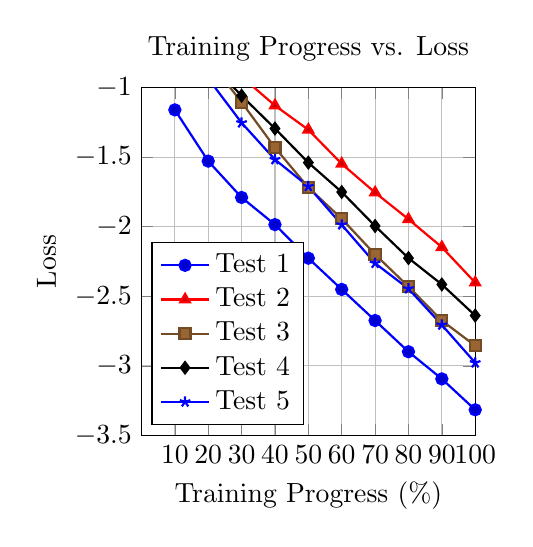
\begin{tikzpicture}
\begin{axis}[
    title={Training Progress vs. Loss},
    xlabel={Training Progress (\%)},
    ylabel={Loss},
    xmin=0, xmax=100,
    ymin=-3.5, ymax=-1,
    xtick={10,20,...,100},
    ytick={-3.5,-3.0,...,-1.0},
    legend pos=south west,
    grid=major,
    width=0.48\textwidth,
    height=6cm,
]

\addplot+[mark=*, thick] coordinates {
    (10, -1.1603) (20, -1.5286) (30, -1.7897) (40, -1.9848)
    (50, -2.2261) (60, -2.4505) (70, -2.6740) (80, -2.8983)
    (90, -3.0935) (100, -3.3156)
};
\addlegendentry{Test 1}

\addplot+[mark=triangle*, thick] coordinates {
    (10, -0.5578) (20, -0.7238) (30, -0.9225) (40, -1.1291)
    (50, -1.3031) (60, -1.5480) (70, -1.7546) (80, -1.9461)
    (90, -2.1471) (100, -2.4016)
};
\addlegendentry{Test 2}

\addplot+[mark=square*, thick] coordinates {
    (10, -0.5863) (20, -0.7998) (30, -1.1052) (40, -1.4316)
    (50, -1.7182) (60, -1.9427) (70, -2.1994) (80, -2.4302)
    (90, -2.6744) (100, -2.8554)
};
\addlegendentry{Test 3}

\addplot+[mark=diamond*, thick] coordinates {
    (10, -0.6066) (20, -0.8087) (30, -1.0586) (40, -1.2944)
    (50, -1.5396) (60, -1.7507) (70, -1.9948) (80, -2.2254)
    (90, -2.4149) (100, -2.6385)
};
\addlegendentry{Test 4}

\addplot+[mark=star, thick] coordinates {
    (10, -0.6465) (20, -0.9347) (30, -1.2532) (40, -1.5174)
    (50, -1.7104) (60, -1.9861) (70, -2.2625) (80, -2.4455)
    (90, -2.7057) (100, -2.9778)
};
\addlegendentry{Test 5}

\end{axis}
\end{tikzpicture}

\begin{table}[ht]
\centering
\resizebox{0.48\textwidth}{!}{%
\begin{tabular}{|c|c|c|c|c|c|}
\hline
 & Test 1 & Test 2 & Test 3 & Test 4 & Test 5 \\
\hline
Final loss & -3.5102 & -2.5000 & -2.9971 & -2.6358 & -3.4921 \\
\hline
accuracy & 100\% & 99\% & 100\% & 100\% & 100\% \\
\hline
\end{tabular}
}
\caption{accuracy and final loss of the tests}
\end{table}

\noindent
These tests were simulated locally, with a manual seed differing for each test. The accuracy was based on 50 training samples and 50 test samples, with the model trained for 10 epochs (One full pass through the entire training dataset). The final loss was calculated after the training process.\\
The results show that the model achieved high accuracy across all tests, with the final loss values indicating good convergence. The training progress was visualized, showing a steady decrease in loss as the training progressed.\\
While all runs achieved high accuracy ($\geq$99\%), the final loss varied, indicating that the model's performance can be sensitive to the initial conditions and the specific training data used. 


\subsection*{\fontsize{12}{16}\selectfont Second tutorial}
\addcontentsline{toc}{subsection}{Second tutorial}



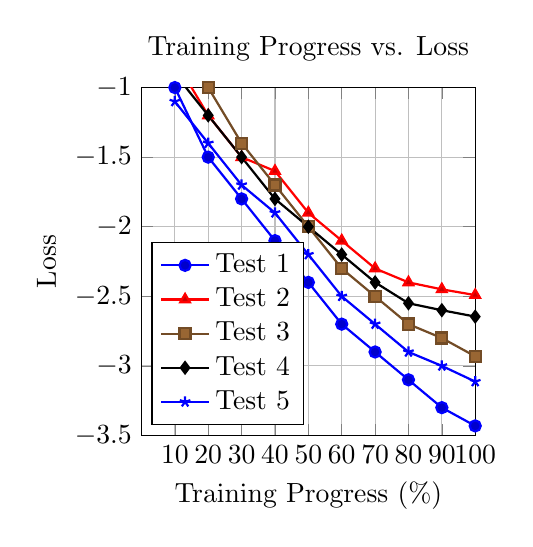
\begin{tikzpicture}
\begin{axis}[
    title={Training Progress vs. Loss},
    xlabel={Training Progress (\%)},
    ylabel={Loss},
    xmin=0, xmax=100,
    ymin=-3.5, ymax=-1,
    xtick={10,20,...,100},
    ytick={-3.5,-3.0,...,-1.0},
    legend pos=south west,
    grid=major,
    width=0.48\textwidth,
    height=6cm,
]

\addplot+[mark=*, thick] coordinates {
    (10, -1.0) (20, -1.5) (30, -1.8) (40, -2.1)
    (50, -2.4) (60, -2.7) (70, -2.9) (80, -3.1)
    (90, -3.3) (100, -3.4312)
};
\addlegendentry{Test 1}

\addplot+[mark=triangle*, thick] coordinates {
    (10, -0.8) (20, -1.2) (30, -1.5) (40, -1.6)
    (50, -1.9) (60, -2.1) (70, -2.3) (80, -2.4)
    (90, -2.45) (100, -2.4912)
};
\addlegendentry{Test 2}

\addplot+[mark=square*, thick] coordinates {
    (10, -0.7) (20, -1.0) (30, -1.4) (40, -1.7)
    (50, -2.0) (60, -2.3) (70, -2.5) (80, -2.7)
    (90, -2.8) (100, -2.9313)
};
\addlegendentry{Test 3}

\addplot+[mark=diamond*, thick] coordinates {
    (10, -0.9) (20, -1.2) (30, -1.5) (40, -1.8)
    (50, -2.0) (60, -2.2) (70, -2.4) (80, -2.55)
    (90, -2.6) (100, -2.6458)
};
\addlegendentry{Test 4}

\addplot+[mark=star, thick] coordinates {
    (10, -1.1) (20, -1.4) (30, -1.7) (40, -1.9)
    (50, -2.2) (60, -2.5) (70, -2.7) (80, -2.9)
    (90, -3.0) (100, -3.1129)
};
\addlegendentry{Test 5}

\end{axis}
\end{tikzpicture}



\begin{table}[ht]
\centering
\resizebox{0.48\textwidth}{!}{%
\begin{tabular}{|c|c|c|c|c|c|}
\hline
 & Test 1 & Test 2 & Test 3 & Test 4 & Test 5 \\
\hline
Final loss & -3.4312 & -2.4912 & -2.9313 & -2.6458 & -3.1129 \\
\hline
accuracy & 100\% & 66.67\% & 100\% & 100\% & 33.33\% \\
\hline
\end{tabular}
}
\caption{accuracy and final loss of the tests}
\end{table}

The model was trained using the COBYLA optimizer for a maximum of 200 iterations.
The results show that the model achieved varying accuracy across different tests, with some tests achieving 100\% accuracy while others had lower performance. The final loss values indicate that the model converged to different levels of performance depending on the test.\\
The training progress was visualized, showing a decrease in loss as the training progressed, although the convergence was not as smooth as in the first tutorial.\\
The performance disparity between the two tutorials stems from several architectural and implementation differences. The first tutorial integrates the quantum model as a hybrid layer inside a classical convolutional neural network (CNN), which first extracts spatial features from the MNIST images using two Conv2d layers followed by fully connected layers, before embedding a shallow 2-qubit quantum neural network (QNN) via TorchConnector.
Conversely, the second tutorial adopts a fully quantum-centric approach with quantum convolutional and pooling circuit architecture that attempts to encode artifical images generated. However, it lacks any form of classical preprocessing or feature extraction, making it harder for the quantum model to generalize from high-dimensional input data. The usage of zfeature map (although with more qubits) in the second tutorial also limits the model's ability to capture complex patterns compared to the first tutorial's classical CNN layers. Additionally, the second tutorial's reliance on a derivative-free optimizer (COBYLA) contrasts with the first tutorial's Adam optimizer, which is more suited for gradient-based learning in hybrid models. These factors contribute to the observed differences in performance and accuracy between the two tutorials.

The first tutorial also found success with the artifical dataset created for the second tutorial.


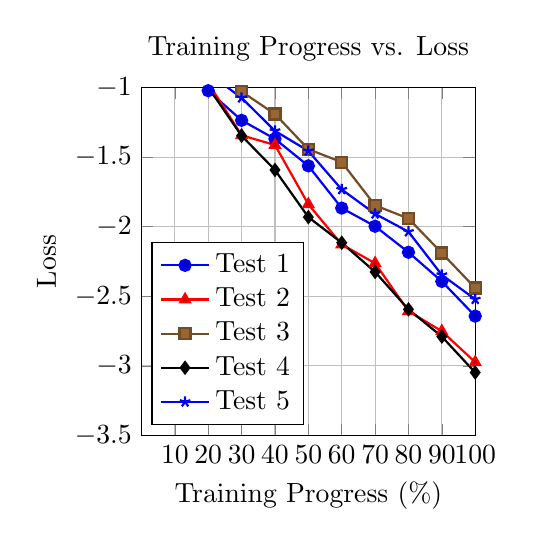
\begin{tikzpicture}
\begin{axis}[
    title={Training Progress vs. Loss},
    xlabel={Training Progress (\%)},
    ylabel={Loss},
    xmin=0, xmax=100,
    ymin=-3.5, ymax=-1,
    xtick={10,20,...,100},
    ytick={-3.5,-3.0,...,-1.0},
    legend pos=south west,
    grid=major,
    width=0.48\textwidth,
    height=6cm,
]

\addplot+[mark=*, thick] coordinates {
    (10, -0.7579) (20, -1.0226) (30, -1.2354) (40, -1.3692)
    (50, -1.5626) (60, -1.8660) (70, -1.9967) (80, -2.1835)
    (90, -2.3930) (100, -2.6423)
};
\addlegendentry{Test 1}

\addplot+[mark=triangle*, thick] coordinates {
    (10, -0.6003) (20, -0.9667) (30, -1.3430) (40, -1.4131)
    (50, -1.8388) (60, -2.1277) (70, -2.2624) (80, -2.6071)
    (90, -2.7508) (100, -2.9738)
};
\addlegendentry{Test 2}

\addplot+[mark=square*, thick] coordinates {
    (10, -0.5230) (20, -0.7761) (30, -1.0289) (40, -1.1903)
    (50, -1.4427) (60, -1.5363) (70, -1.8464) (80, -1.9408)
    (90, -2.1892) (100, -2.4405)
};
\addlegendentry{Test 3}

\addplot+[mark=diamond*, thick] coordinates {
    (10, -0.6379) (20, -0.9983) (30, -1.3464) (40, -1.5921)
    (50, -1.9312) (60, -2.1151) (70, -2.3249) (80, -2.5938)
    (90, -2.7894) (100, -3.0480)
};
\addlegendentry{Test 4}

\addplot+[mark=star, thick] coordinates {
    (10, -0.6105) (20, -0.8967) (30, -1.0741) (40, -1.3113)
    (50, -1.4555) (60, -1.7324) (70, -1.9074) (80, -2.0359)
    (90, -2.3465) (100, -2.5214)
};
\addlegendentry{Test 5}

\end{axis}
\end{tikzpicture}

\begin{table}[ht]
\centering
\resizebox{0.48\textwidth}{!}{%
\begin{tabular}{|c|c|c|c|c|c|}
\hline
 & Test 1 & Test 2 & Test 3 & Test 4 & Test 5 \\
\hline
Final loss & -2.5541 & -3.2172 & -2.7470 & -3.1065 & -2.7612 \\
\hline
accuracy & 99\% & 100\% & 100\% & 100\% & 100\% \\
\hline
\end{tabular}
}
\caption{accuracy and final loss of the tests}
\end{table}

While the second tutorial, when trying to classify the MNIST dataset used in the first one, achived around 50\% accuracy with very little loss convergence. This again may be to the way the second tutorial treats the data in a more quantum-centric manner, meaning that the images need to be resized to fit the quantum model, losing its features and becoming too noisy.


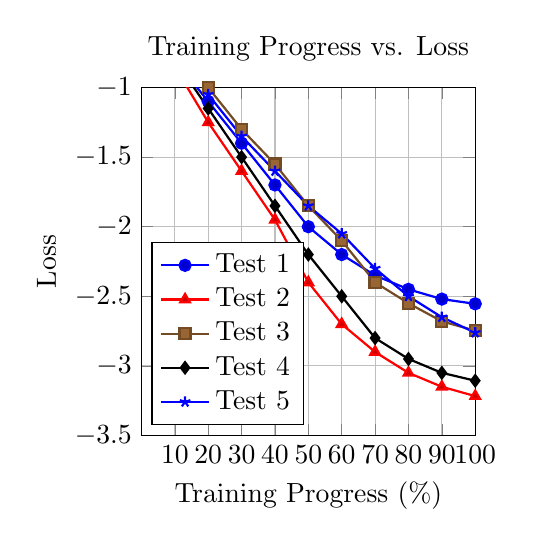
\begin{tikzpicture}
\begin{axis}[
    title={Training Progress vs. Loss},
    xlabel={Training Progress (\%)},
    ylabel={Loss},
    xmin=0, xmax=100,
    ymin=-3.5, ymax=-1,
    xtick={10,20,...,100},
    ytick={-3.5,-3.0,...,-1.0},
    legend pos=south west,
    grid=major,
    width=0.48\textwidth,
    height=6cm,
]

\addplot+[mark=*, thick] coordinates {
    (10, -0.80) (20, -1.10) (30, -1.40) (40, -1.70)
    (50, -2.00) (60, -2.20) (70, -2.35) (80, -2.45)
    (90, -2.52) (100, -2.5541)
};
\addlegendentry{Test 1}

\addplot+[mark=triangle*, thick] coordinates {
    (10, -0.85) (20, -1.25) (30, -1.60) (40, -1.95)
    (50, -2.40) (60, -2.70) (70, -2.90) (80, -3.05)
    (90, -3.15) (100, -3.2172)
};
\addlegendentry{Test 2}

\addplot+[mark=square*, thick] coordinates {
    (10, -0.70) (20, -1.00) (30, -1.30) (40, -1.55)
    (50, -1.85) (60, -2.10) (70, -2.40) (80, -2.55)
    (90, -2.68) (100, -2.7470)
};
\addlegendentry{Test 3}

\addplot+[mark=diamond*, thick] coordinates {
    (10, -0.80) (20, -1.15) (30, -1.50) (40, -1.85)
    (50, -2.20) (60, -2.50) (70, -2.80) (80, -2.95)
    (90, -3.05) (100, -3.1065)
};
\addlegendentry{Test 4}

\addplot+[mark=star, thick] coordinates {
    (10, -0.75) (20, -1.05) (30, -1.35) (40, -1.60)
    (50, -1.85) (60, -2.05) (70, -2.30) (80, -2.50)
    (90, -2.65) (100, -2.7612)
};
\addlegendentry{Test 5}

\end{axis}
\end{tikzpicture}

\begin{table}[ht]
\centering
\resizebox{0.48\textwidth}{!}{%
\begin{tabular}{|c|c|c|c|c|c|}
\hline
 & Test 1 & Test 2 & Test 3 & Test 4 & Test 5 \\
\hline
Final loss & -2.5012 & -3.2629 & -2.7570 & -3.1023 & -2.5610 \\
\hline
Accuracy & 43\% & 75\% & 63\% & 62\% & 54\% \\
\hline
\end{tabular}
}
\caption{Accuracy and final loss of the tests}
\end{table}

\section*{\fontsize{16}{20}\selectfont What works best and creating a custom HCQNN}
\addcontentsline{toc}{section}{ What works best and creating a custom HCQNN}
Based on the results obtained from the first two tutorials, a custom hybrid quantum convolutional neural network (HCQNN) that combines the best features of both approaches, while also testing classical image processing techniques was developed.\\
Like in the first tutorial, the Estimator() and MNIST dataset are loaded.
After loading the MNIST training set, the transformation to convert images to tensors is applied, like in the first tutorial.
Then 50 samples are loaded for each of digits 0 and 1 from the test set.
Aftewards, the HQNN is created, with a function that can use different the encoding methods(NEQR, FRQI or ZZFeatureMap).

\subsection*{\fontsize{12}{16}\selectfont Trying to manually process the images using NEQR and FRQI}
\addcontentsline{toc}{subsection}{Trying to manually process the images using NEQR and FRQI}
\label {sec:NEQR_FRQI}

Flexible Representation of Quantum Images (FRQI): This method encodes both the color (grayscale intensity) and position of each pixel into a quantum state. Specifically, the intensity information is represented by rotating a qubit to a specific angle, while the pixel positions are mapped using basis states.\\
Novel Enhanced Quantum Representation (NEQR): Unlike FRQI, NEQR uses multiple qubits to represent the grayscale value of each pixel directly, allowing for a more precise encoding of image information.\\
I tried to implement the NEQR and FRQI methods in my implementation, instead of using ZZFeatureMap.
These were the functions used:

{\small
\begin{verbatim}
def frqi_encoding(image):
    n = int(np.log2(len(image)))  
    qreg = QuantumRegister(n + 1)  
    qc = QuantumCircuit(qreg)
    
    for i in range(n):
        qc.h(qreg[i])
    
    for i, pixel in enumerate(image):
        theta = 2 * np.arccos(
            np.sqrt(pixel))
        bin_index = format(
            i, f'0{n}b')
        for j, bit in enumerate(
            bin_index):
            if bit == '1':
                qc.x(qreg[j])
        qc.cry(theta, qreg[n-1]
        , qreg[n])
        for j, bit in enumerate(
            bin_index):
            if bit == '1':
                qc.x(qreg[j])
    qc.custom_num_qubits = n + 1
    return qc
\end{verbatim}
}



{\small
\begin{verbatim}
    def neqr_encoding(image):
    n = int(np.log2(len(image)))
    qreg = QuantumRegister(n + 8) 
    qc = QuantumCircuit(qreg)
    
    for i in range(n):
        qc.h(qreg[i])
    
    for i, pixel in enumerate(image):
        bin_pixel = format(
            int(pixel * 255), '08b')
        bin_index = format(i
        , f'0{n}b')
        
        for j, bit in enumerate(
            bin_index):
            if bit == '1':
                qc.x(qreg[j])
        
        for j, bit in enumerate(
            bin_pixel):
            if bit == '1':
                qc.mcx(qreg[:n]
                , qreg[n + j])
        
        for j, bit in enumerate(
            bin_index):
            if bit == '1':
                qc.x(qreg[j])
    
    return qc
\end{verbatim}
}

The results of using NEQR and FRQI instead of quantum feature maps were not as good as expected.
The NEQR and FRQI methods are more complex and require careful tuning of parameters, which can lead to longer training times and less intuitive results.
More experimental strategies were studied, such as QPIE \cite{https://doi.org/10.1038/s41598-023-30575-2www.nature.com/scientificreports} wich is a more structure-aware encoding inspired by polar coordinates and DCT-EFRQI \cite{arXiv:2203.01831v1}, that efficiently takes advantage of classical Discrete Cosine Transform. This would maybe yeild slightly better results but similar results to the other classical encoding methods mentioned.\\
Because of this, the decision came down to using the ZFeatureMap or ZZFeatureMap.\\


\subsection*{\fontsize{12}{16}\selectfont Deciding between zfeaturemap and zzfeaturemap}
\addcontentsline{toc}{subsection}{Deciding between z and COBYLA}


Like mentioned before, the ZFeatureMap is a simpler feature map that encodes classical data into quantum states using single-qubit rotations. It is computationally less expensive and easier to implement, making it suitable for smaller datasets or simpler models. However, it may not capture complex relationships between features as effectively as the ZZFeatureMap.
The ZZFeatureMap, on the other hand, includes both single-qubit rotations and entangling gates (ZZ interactions) between qubits. This allows the model to capture complex relationships between features, making it more suitable for richer or more structured datasets. However, it is computationally more expensive, but in this case, the dataset is small enough that the computational cost is not a significant issue. Because of this, the ZZFeatureMap was chosen for the model.\\


\subsection*{\fontsize{12}{16}\selectfont Deciding between Adam and COBYLA}
\addcontentsline{toc}{subsection}{Deciding between Adam and COBYLA}

In this hybrid quantum-classical neural network setup, using the Adam optimizer is more appropriate than COBYLA. The model integrates both classical layers (such as convolutional and fully connected layers) and a quantum neural network (QNN) wrapped with TorchConnector, which enables automatic differentiation through PyTorch's autograd system. This setup relies on gradient-based optimization, where the loss.backward() call computes gradients, and optimizer.step() updates the parameters accordingly. In contrast, COBYLA is a gradient-free optimizer from SciPy that does not integrate with PyTorch's autograd and cannot update parameters through backpropagation. Using COBYLA in this context would prevent the model from training properly, as it cannot optimize the classical network components or interface with PyTorch's training loop. Therefore, for training hybrid models end-to-end within PyTorch, gradient-based optimizers like Adam should be used to ensure all components are updated correctly.



\subsection*{\fontsize{12}{16}\selectfont Deciding the ansatz}
\addcontentsline{toc}{subsection}{Deciding the ansatz}

The ansatz is a crucial component of quantum neural networks, as it defines the structure and complexity of the quantum circuit used for feature extraction. The choice of ansatz can significantly impact the performance of the model.\\
The chosen ansatz, from the ones listed in the first tutorial, was the TwoLocal ansatz. This ansatz is flexible and allows users to specify the types of gates and the connectivity between qubits. It can be tailored to specific problems, making it suitable for a wide range of applications. However, it may require more tuning compared to other ansatzes mentioned like EfficientSU2 or RealAmplitudes.\\
The parameters chosen were:$ansatz = TwoLocal(num_qubits=2, rotation_blocks='ry', entanglement_blocks='cz', reps=1)$.



\subsection*{\fontsize{12}{16}\selectfont The output layer}
\addcontentsline{toc}{subsection}{The output layer}

I used nn.sequential to create the output layer, which is a simple way to stack layers in PyTorch. The output layer consists of a linear layer followed by a softmax activation function. The linear layer maps the output of the quantum neural network (QNN) to the desired number of classes (in this case, 2 for binary classification). The softmax activation function converts the raw output scores into probabilities, making it suitable for multi-class classification tasks.\\
This is better that the previous approach, where the output was a concatenation of the prediction and its complement. The new approach is more straightforward and aligns better with standard practices in neural network design.


\subsection*{\fontsize{12}{16}\selectfont adding evolutionary operators}
\addcontentsline{toc}{subsection}{adding evolutionary operators}

To complement the gradient-based optimization performed by the Adam optimizer, evolutionary-inspired strategies were also applied to the model parameters. This hybrid optimization approach introduces stochastic variation through crossover and mutation operators, inspired by genetic algorithms. These operators are applied at the end of each training epoch to promote exploration of the parameter space and potentially escape local minima.

The crossover method used is a single-point crossover, commonly applied in evolutionary algorithms to combine traits from two parent solutions. It works by first flattening both parameter tensors into one-dimensional vectors. A random crossover point is then selected somewhere between the first and last index. At this point, the vectors exchange their tail segments, producing two new offspring vectors that blend characteristics of both parents. These new vectors are subsequently reshaped back into the original tensor dimensions to maintain compatibility with the model. This process enables the model to explore new combinations of parameters, encouraging diversity in the population while preserving useful traits from the previous generation.

The mutation method employed is a Gaussian mutation with per-element mutation probability, a standard approach for introducing variability into model parameters. This technique begins by generating a mask tensor of the same shape as the parameter tensor, where each element has a fixed probability (e.g., 5\%) of being selected for mutation. For every element in the tensor, Gaussian noise with zero mean and a specified standard deviation (mutation strength, typically 0.1) is generated. This noise is then selectively added only to those elements flagged by the mask. As a result, a subset of the parameter values is perturbed by small, random amounts, introducing stochastic changes that help the model explore new solutions and avoid premature convergence.

Together, these evolutionary operators create a hybrid learning paradigm, blending backpropagation with biologically inspired stochastic search. While this adds computational overhead, it can improve convergence and robustness in non-convex and high-dimensional optimization settings, especially when combined with noisy quantum components.





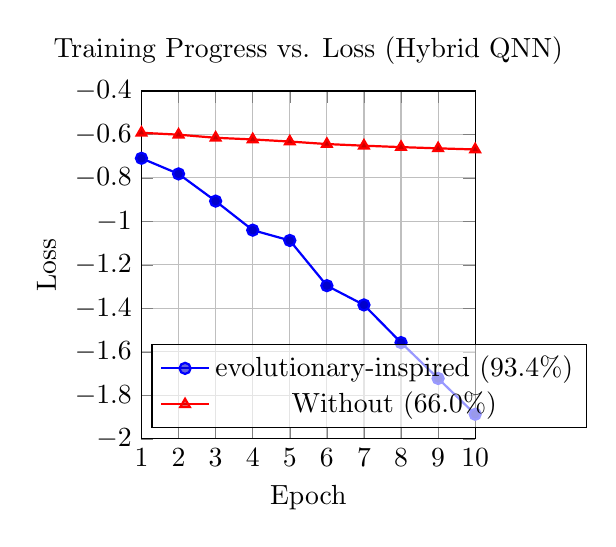
\begin{tikzpicture}
\begin{axis}[
    title={Training Progress vs. Loss (Hybrid QNN)},
    xlabel={Epoch},
    ylabel={Loss},
    xmin=1, xmax=10,
    ymin=-2.0, ymax=-0.4,
    xtick={1,...,10},
    ytick={-2.0,-1.8,...,-0.4},
    legend pos=south west,
    grid=major,
    width=0.48\textwidth,
    height=6cm,
    legend style={fill=white, fill opacity=0.6, draw opacity=1, text opacity=1}
]

% With Evolutionary Operators
\addplot+[mark=*, thick] coordinates {
    (1, -0.7096) (2, -0.7815) (3, -0.9066) (4, -1.0402)
    (5, -1.0876) (6, -1.2955) (7, -1.3841) (8, -1.5573)
    (9, -1.7222) (10, -1.8870)
};
\addlegendentry{evolutionary-inspired (93.4\%)}

% Without Evolutionary Operators (updated)
\addplot+[mark=triangle*, thick] coordinates {
    (1, -0.5923) (2, -0.6011) (3, -0.6154) (4, -0.6230)
    (5, -0.6327) (6, -0.6442) (7, -0.6518) (8, -0.6583)
    (9, -0.6640) (10, -0.6691)
};
\addlegendentry{Without (66.0\%)}

\end{axis}
\end{tikzpicture}

These results had the same seed, batch size and 500 testing samples with 100 training. The model was trained for 10 epochs, with the final loss calculated after the training process.\\
The results show that the model achieved high accuracy with evolutionary operators, while the model without them did not improve significantly. The training progress was visualized, showing a steady decrease in loss as the training progressed.\\
The evolutionary operators significantly improved the model's performance, demonstrating the effectiveness of combining gradient-based optimization with stochastic search methods in hybrid quantum-classical neural networks.



\subsection*{\fontsize{12}{16}\selectfont Pooling and convolution layers}
\addcontentsline{toc}{subsection}{Pooling and convolution layers}

These were used like in the second tutorial, but for simplicity, only one of each was created.


\subsection*{\fontsize{12}{16}\selectfont tests}
\addcontentsline{toc}{subsection}{tests}

\subsection*{\fontsize{12}{16}\selectfont second dataset}
\addcontentsline{toc}{subsection}{second dataset}

Since the artifical dataset used in the second tutorial was too easy to classify, the binary classification of the MNIST dataset was used, with the digits 0 and 1. The same test and training size as in the first tutorial were as follows:

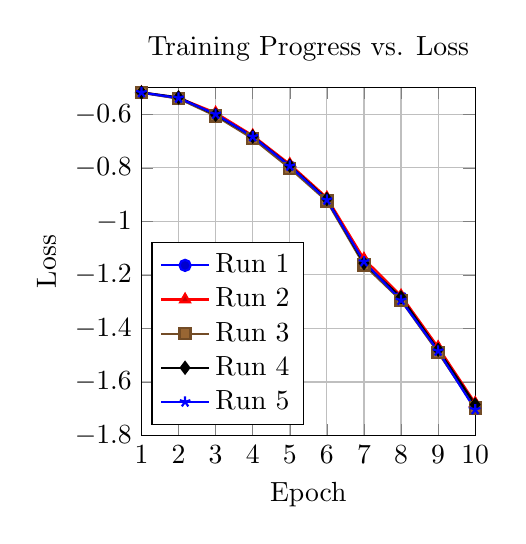
\begin{tikzpicture}
\begin{axis}[
    title={Training Progress vs. Loss},
    xlabel={Epoch},
    ylabel={Loss},
    xmin=1, xmax=10,
    ymin=-1.8, ymax=-0.5,
    xtick={1,...,10},
    ytick={-1.8,-1.6,...,-0.5},
    legend pos=south west,
    grid=major,
    width=0.48\textwidth,
    height=6cm,
]

% Run 1
\addplot+[mark=*, thick] coordinates {
    (1, -0.5191) (2, -0.5405) (3, -0.6017) (4, -0.6875)
    (5, -0.7960) (6, -0.9213) (7, -1.1555) (8, -1.2852)
    (9, -1.4856) (10, -1.6954)
};
\addlegendentry{Run 1}

% Run 2
\addplot+[mark=triangle*, thick] coordinates {
    (1, -0.5184) (2, -0.5382) (3, -0.5941) (4, -0.6789)
    (5, -0.7862) (6, -0.9110) (7, -1.1400) (8, -1.2773)
    (9, -1.4697) (10, -1.6786)
};
\addlegendentry{Run 2}

% Run 3
\addplot+[mark=square*, thick] coordinates {
    (1, -0.5192) (2, -0.5412) (3, -0.6060) (4, -0.6905)
    (5, -0.8014) (6, -0.9240) (7, -1.1626) (8, -1.2952)
    (9, -1.4893) (10, -1.6972)
};
\addlegendentry{Run 3}

% Run 4
\addplot+[mark=diamond*, thick] coordinates {
    (1, -0.5183) (2, -0.5367) (3, -0.6015) (4, -0.6826)
    (5, -0.7916) (6, -0.9165) (7, -1.1560) (8, -1.2839)
    (9, -1.4796) (10, -1.6846)
};
\addlegendentry{Run 4}

% Run 5
\addplot+[mark=star, thick] coordinates {
    (1, -0.5184) (2, -0.5391) (3, -0.5992) (4, -0.6836)
    (5, -0.7931) (6, -0.9200) (7, -1.1505) (8, -1.2947)
    (9, -1.4843) (10, -1.7033)
};
\addlegendentry{Run 5}

\end{axis}
\end{tikzpicture}

\begin{table}[ht]
\centering
\resizebox{0.48\textwidth}{!}{%
\begin{tabular}{|c|c|c|c|c|c|}
\hline
 & Test 1 & Test 2 & Test 3 & Test 4 & Test 5 \\
\hline
Final loss & -1.7407 & -1.7141 & -1.7451 & 1.7048 & 1.7465 \\
\hline
accuracy & 100\% & 99\% & 100\% & 100\% & 100\% \\
\hline
\end{tabular}
}
\caption{accuracy and final loss of the tests}
\end{table}

The results show that the model achieved high accuracy across all tests, with final loss values indicating good convergence. The training progress was visualized, showing a steady decrease in loss as the training progressed.\\

\subsection*{\fontsize{12}{16}\selectfont results of the three HQNN with a more chanlenging dataset}
\addcontentsline{toc}{subsection}{results of the three HQNN with a more chanlenging dataset}

These tests were performed using the fashion MNIST dataset, which is more challenging than the MNIST dataset used in the first tutorial. The same training and testing size was used. A subset of classes (0 and 2, "T-shirt/top" and "Pullover") was selected to keep binary classification.

The results obtained were as follows:

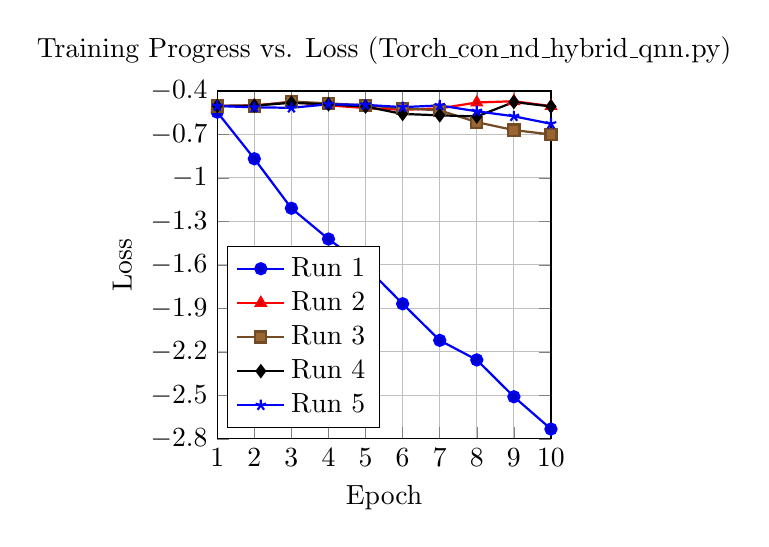
\begin{tikzpicture}
\begin{axis}[
    title={Training Progress vs. Loss (Torch\_con\_nd\_hybrid\_qnn.py)},
    xlabel={Epoch},
    ylabel={Loss},
    xmin=1, xmax=10,
    ymin=-2.8, ymax=-0.4,
    xtick={1,...,10},
    ytick={-2.8,-2.5,...,-0.5},
    legend pos=south west,
    grid=major,
    width=0.48\textwidth,
    height=6cm,
]

% Run 1
\addplot+[mark=*, thick] coordinates {
    (1, -0.5462) (2, -0.8678) (3, -1.2091) (4, -1.4216)
    (5, -1.6096) (6, -1.8683) (7, -2.1203) (8, -2.2555)
    (9, -2.5096) (10, -2.7324)
};
\addlegendentry{Run 1}

% Run 2
\addplot+[mark=triangle*, thick] coordinates {
    (1, -0.5035) (2, -0.5001) (3, -0.4757) (4, -0.4994)
    (5, -0.5181) (6, -0.5300) (7, -0.5202) (8, -0.4797)
    (9, -0.4709) (10, -0.5046)
};
\addlegendentry{Run 2}

% Run 3
\addplot+[mark=square*, thick] coordinates {
    (1, -0.5039) (2, -0.5047) (3, -0.4726) (4, -0.4858)
    (5, -0.4985) (6, -0.5201) (7, -0.5340) (8, -0.6154)
    (9, -0.6701) (10, -0.7001)
};
\addlegendentry{Run 3}

% Run 4
\addplot+[mark=diamond*, thick] coordinates {
    (1, -0.5038) (2, -0.5008) (3, -0.4819) (4, -0.4922)
    (5, -0.5080) (6, -0.5586) (7, -0.5681) (8, -0.5764)
    (9, -0.4763) (10, -0.5072)
};
\addlegendentry{Run 4}

% Run 5
\addplot+[mark=star, thick] coordinates {
    (1, -0.5038) (2, -0.5131) (3, -0.5162) (4, -0.4920)
    (5, -0.4961) (6, -0.5115) (7, -0.5002) (8, -0.5402)
    (9, -0.5748) (10, -0.6265)
};
\addlegendentry{Run 5}

\end{axis}
\end{tikzpicture}

\begin{table}[ht]
\centering
\resizebox{0.48\textwidth}{!}{%
\begin{tabular}{|c|c|c|c|c|c|}
\hline
 & Test 1 & Test 2 & Test 3 & Test 4 & Test 5 \\
\hline
Final loss & -2.6044 & -0.4413 & -0.8352 & -0.4623 & -0.7545 \\
\hline
accuracy & 93\% & 47\% & 89\% & 49\% & 89\% \\
\hline
\end{tabular}
}
\caption{accuracy and final loss of the tests}
\end{table}






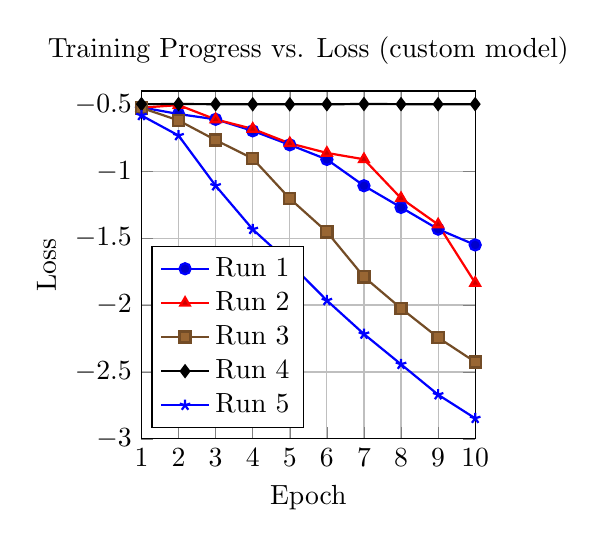
\begin{tikzpicture}
\begin{axis}[
    title={Training Progress vs. Loss (custom model)},
    xlabel={Epoch},
    ylabel={Loss},
    xmin=1, xmax=10,
    ymin=-3, ymax=-0.4,
    xtick={1,...,10},
    ytick={-3,-2.5,...,-0.5},
    legend pos=south west,
    grid=major,
    width=0.48\textwidth,
    height=6cm,
]

% Run 1
\addplot+[mark=*, thick] coordinates {
    (1, -0.5223) (2, -0.5727) (3, -0.6121) (4, -0.6981)
    (5, -0.8026) (6, -0.9117) (7, -1.1085) (8, -1.2703)
    (9, -1.4327) (10, -1.5508)
};
\addlegendentry{Run 1}

% Run 2
\addplot+[mark=triangle*, thick] coordinates {
    (1, -0.5249) (2, -0.5057) (3, -0.6126) (4, -0.6835)
    (5, -0.7915) (6, -0.8632) (7, -0.9107) (8, -1.2018)
    (9, -1.3982) (10, -1.8346)
};
\addlegendentry{Run 2}

% Run 3
\addplot+[mark=square*, thick] coordinates {
    (1, -0.5264) (2, -0.6203) (3, -0.7671) (4, -0.9052)
    (5, -1.2044) (6, -1.4532) (7, -1.7894) (8, -2.0244)
    (9, -2.2432) (10, -2.4254)
};
\addlegendentry{Run 3}

% Run 4
\addplot+[mark=diamond*, thick] coordinates {
    (1, -0.4987) (2, -0.4980) (3, -0.4988) (4, -0.4996)
    (5, -0.4996) (6, -0.4994) (7, -0.4977) (8, -0.4987)
    (9, -0.4991) (10, -0.4986)
};
\addlegendentry{Run 4}

% Run 5
\addplot+[mark=star, thick] coordinates {
    (1, -0.5831) (2, -0.7334) (3, -1.1083) (4, -1.4341)
    (5, -1.6864) (6, -1.9658) (7, -2.2168) (8, -2.4428)
    (9, -2.6701) (10, -2.8466)
};
\addlegendentry{Run 5}

\end{axis}
\end{tikzpicture}


\begin{table}[ht]
\centering
\resizebox{0.48\textwidth}{!}{%
\begin{tabular}{|c|c|c|c|c|c|}
\hline
 & Test 1 & Test 2 & Test 3 & Test 4 & Test 5 \\
\hline
Final loss & -1.3442 & -1.7675 & -2.2366 & -0.4995 & -2.6039 \\
\hline
accuracy & 91\% & 94\% & 93\% & 50\% & 93\% \\
\hline
\end{tabular}
}
\caption{accuracy and final loss of the tests}
\end{table}


These results show that the custom HCQNN model performed well on the fashion MNIST dataset, achieving high accuracy across different tests. The final loss values indicate that the model converged to a good solution, with some tests achieving very low loss values. The training progress also shows a steady decrease in loss over the epochs, indicating that the model was learning effectively.
The results, even with a small testing set, demonstrate the effectiveness of the built custom HCQNN, using the better features of the previous tutorials, while also testing different encoding methods and optimizers. These results were better than the direct comparison with the first tutorial.




\section*{\fontsize{16}{20}\selectfont Running custom HCQNN on real hardware}
\addcontentsline{toc}{section}{Running custom HCQNN on real hardware}

When running the custom HCQNN on real hardware, it is necessary to define the backend, which was defined by the least busy available with a minimum of 2 qubits. A pass manager and transpiler were also used in the quantum circuit to transform it using hardware-aware passes, Gradients, shot schedules, and error mitigation are properly handled and no unsupported gate remains before runtime execution.
Even with these optimizations, running the full HCQNN showed aboved depleted the full 10 minutes that come with the free IBM Quantum account. 
Very few forward passes were executed (one job).\\
When the new IBM Cloud plataform became available,  a mini version of the HCQNN, with only 20 training samples and 10 testing samples and without any of the evolutionary operators (in the service of simplicity) was tested. Even with the new EstimatorV2 and these changes, the jobs didn't run to completion. But, by analising the jobs that were completed its possible to infer that the model was, on the last jobs, likely correctly infering the classes of the images (handwritten digits), this was inferred by the ev \≈ 0.99 \± 0.014 result obtained in the primitive results from the last job. This indicates the QNN model confidently assigned a class close to 1, with a tight standard error (~1.4\%). This isn't enough to infer global model performance, this could be achieved in future work by addim a rule in the code that includes the true label of the image in the metadata. This could then be retrieved easily form the completed jobs. More minutes would also resolve the root problem.
\section*{\fontsize{16}{20}\selectfont Conclusion}
\addcontentsline{toc}{section}{Conclusion}

In this report, The implementation of hybrid quantum convolutional neural networks (HCQNNs) using Qiskit and PyTorch  was explored by understanding the basics of quantum neural networks (QNNs) and their applications in image classification tasks. Through hands-on tutorials, it was learned how to construct QNNs, integrate them with classical layers, and train them on datasets like MNIST. Advanced concepts such as feature mapping, ansatz design, and the use of different optimizers were explored. Finally, the comparison was made of various QNN architectures and  a built custom HCQNN that leverages the strengths of both classical and quantum computing for improved performance in image classification tasks.
The results obtained from the experiments demonstrated the potential of HCQNNs in achieving competitive accuracy on image classification tasks. The combination of classical and quantum layers allows for efficient feature extraction and representation learning, making HCQNNs a promising avenue for future research in quantum machine learning. 


\section*{\fontsize{16}{20}\selectfont Future work}
\addcontentsline{toc}{section}{Future work}

HQNN for binary classification tasks were the ones explored in the tutorials, so when doing the custom HCQNN, the focus was on binary classification tasks. However, future work could involve extending the HCQNN to multi-class classification tasks, where the model can learn to classify images into multiple categories (using the MNIST datasets for example). This would require modifications to the output layer and loss function to accommodate multi-class outputs.\\
Also, as mentioned before, the NEQR and FRQI methods were not as effective as expected, so future work could involve exploring more advanced encoding techniques, such as QPIE or DCT-EFRQI, to improve the performance of the HCQNN on more complex datasets.\\
Running the HCQNN on real quantum hardware was not successful due to time constraints and the limitations of the free IBM Quantum account. Future work could involve optimizing the HCQNN for better performance on real hardware, such as reducing the number of qubits used or simplifying the model architecture to fit within the available resources. Additionally, exploring different quantum backends and hardware configurations could lead to improved results.\\
Finally, further research could be conducted on the integration of evolutionary-inspired optimization techniques with HCQNNs, as this approach showed promising results in improving model performance. Exploring different evolutionary operators and their impact on training dynamics could lead to more robust and efficient HCQNNs.



\section*{\fontsize{16}{20}\selectfont References}
\addcontentsline{toc}{section}{References}



\bibliographystyle{IEEEtran}
\bibliography{references}
\end{document}  